%%
%% LinkedListLab (c) 2021-24 Christopher A. Bohn
%%
%% Assignment writeup licensed under the Creative Commons Attribution 4.0 International License
%% https://creativecommons.org/licenses/by/4.0/
%%

\documentclass[12pt]{article}
\usepackage{booktabs}

%%
%% labs/common/assignment.tex
%% (c) 2021-23 Christopher A. Bohn
%%
%% Licensed under the Apache License, Version 2.0 (the "License");
%% you may not use this file except in compliance with the License.
%% You may obtain a copy of the License at
%%     http://www.apache.org/licenses/LICENSE-2.0
%% Unless required by applicable law or agreed to in writing, software
%% distributed under the License is distributed on an "AS IS" BASIS,
%% WITHOUT WARRANTIES OR CONDITIONS OF ANY KIND, either express or implied.
%% See the License for the specific language governing permissions and
%% limitations under the License.
%%

\usepackage{addfont}
\usepackage{amsmath}
\usepackage{amssymb}
\usepackage{animate}
\usepackage{bold-extra}
\usepackage{cancel}
\usepackage{caption}
\usepackage{ccicons}
\usepackage{enumitem}
\usepackage{etoolbox}
\usepackage{fancyhdr}
\usepackage{fullpage}
\usepackage{graphicx}
\usepackage{hyperref}
\usepackage[utf8]{inputenc}
\usepackage[procnames]{listings}
%\usepackage{media9}
\usepackage{multicol}
\usepackage{subfig}
\usepackage{textcomp}
\usepackage{tikz}
\usepackage[americanresistor]{circuitikz}
\usepackage{tikz-uml}
\usetikzlibrary{automata,positioning,arrows}
\usepackage[normalem]{ulem}
\usepackage{wrapfig}
\usepackage{xcolor}
%\usepackage[dvipsnames]{xcolor}

\lstset{language=C, tabsize=4, upquote=true, basicstyle=\ttfamily}
\newcommand{\function}[1]{\textbf{\lstinline{#1}}}
\setlength{\headsep}{0.7cm}
\hypersetup{colorlinks=true}

%% CREDIT FOR MARKERLESSFOOTNOTE WHERE CREDIT IS DUE: https://tex.stackexchange.com/questions/30720/footnote-without-a-marker?answertab=scoredesc#tab-top
\newcommand\markerlessfootnote[1]{%
    \begingroup
    \renewcommand\thefootnote{}\footnote{#1}%
    \addtocounter{footnote}{-1}%
    \endgroup
}

\newcommand{\pagelayout}{
    \pagestyle{fancy}
    \fancyhf{}
    \lhead{\coursenumber}
    \chead{\ Lab \labnumber: \labname}
    \rhead{\courseterm}
    \cfoot{\shortlabname-\thepage}
}

\newcommand{\labidentifier}{
    \title{\ Lab \labnumber}
    \author{\labname}
    \date{Due: \duedate}
    \maketitle

    \textit{\collaborationrules}
    \markerlessfootnote{\tiny{\ifdefstring{\instructorname}{Christopher A. Bohn}{Assignment}{Original assignment} and starter code \copyright\ Christopher A. Bohn, licensed under the Creative Commons Attribution 4.0 International License~\ccby\ and under the Apache License Version 2.0, respectively.}}
    \ifdefstring{\instructorname}{Christopher A. Bohn}{}{\markerlessfootnote{\tiny{Configured for \coursenumber\ at \institutename\ by \instructorname.}}}

    \begin{description}
        \item[Obtaining the starter code] \filesource
        \item[Runtime environment] We will grade this assignment by compiling and running it on \runtimeenvironment;
            you should compile and test your code on \runtimeenvironment\ before turning it in.
        \item[Submitting your work] \filesubmission
    \end{description}
}

% display module fonts for hardware kit
% use with the Capital baseball "matrix printer" font collection (https://www.ctan.org/tex-archive/fonts/capbas/)
% Identifying the specific font in the assignment sheet is deprecated
%   -- instead, set the `usedisplayfont` boolean and the `displaymodule` variable in semester.tex,
%      and \display{...} in the assignment sheet

\addfont{OT1}{d7seg}{\dviiseg}
\addfont{OT1}{deseg}{\deseg}
\addfont{OT1}{necker}{\necker}

\providebool{usedisplayfont}

\newcommand{\display}[1]{
    \ifboolexpe{bool{usedisplayfont}}{
        \ifdefstring{\displaymodule}{MAX7219digits}{{\dviiseg #1}}{}
        \ifdefstring{\displaymodule}{MAX7219matrix}{{\deseg #1}}{}
        \ifdefstring{\displaymodule}{LCD1602}{{\necker #1}}{}
        % We don't yet have a Cow Pi configuration with 14-segment displays, so no \deseg yet
    }{
        \texttt{#1}
    }
}

\newcommand{\rubricitem}[2]{\item[\underline{\hspace{1cm}} +#1] #2}
\newcommand{\bonusitem}[2]{\item[\underline{\hspace{1cm}} Bonus +#1] #2}
\newcommand{\penaltyitem}[2]{\item[\underline{\hspace{1cm}} -#1] #2}
\newcommand{\checkoffitem}[1]{\item (\phantom{xxx}) #1}
\newcommand{\precheckoffitem}[1]{\item [] (\phantom{xxx}) #1}
../../common/assignment/linked-list-nodes.tex

\lstset{language=c, numbers=left, showstringspaces=false,
    moredelim = [s][\ttfamily]{/*}{*/} % I shouldn't need this parameter!
}
%%
%%
% Credit where credit is due. Skipping line numbers from
% https://tex.stackexchange.com/questions/476100/lstlisting-line-number-gaps
\makeatletter
\let\orig@lstnumber=\thelstnumber

\newcommand\lstsetnumber[1]{\gdef\thelstnumber{#1}}
\newcommand\lstresetnumber{\global\let\thelstnumber=\orig@lstnumber}
\makeatother
%%
%%


\pagelayout
\begin{document}
    \labidentifier

    \pdfbookmark[1]{Frontmatter}{frontmatter}                       In this assignment, you will write code for \runtimeenvironment\ that will use new electronic devices to interact with the physical world.

The instructions are written assuming you will edit the code in the Arduino IDE and run it on \runtimeenvironment, constructed according to the pre-lab instructions.
If you wish, you may edit the code in a different environment; however, our ability to provide support for problems with other IDEs is limited.

\section*{Learning Objectives}

After successful completion of this assignment, students will be able to:
\begin{itemize}
    \item Work collaboratively on a hardware/software project
    \item Design and implement a simple embedded system
    \item Expand their programming knowledge by consulting documentation
\end{itemize}

\subsection*{Continuing Forward}

This penultimate lab assignment does not contribute to the final lab assignment.
By integrating elements of what you learned in this course, and by demonstrating that you can review documentation to learn on your own, to design a small embedded system, you will show how much progress you have made this semester.

\section*{During Lab Time}

During your lab period, coordinate with your group partner(s) to decide on your working arrangements.
Unless you're only going to work on the assignment when you're together, you may want to set up a private Git repository that is shared with your partner(s).
With your partner(s), modify your hardware kit as described in Section~\ref{sec:hardwareMods}.
Then, think through your system's design and begin implementing it.
The TAs will be available for questions.


    \softwareengineeringfrontmatter

    \section*{Scenario}                                             \scenariointroduction

    \section{Assignment Summary}                                    This assignment is principally about getting comfortable when explicitly working with memory.
Being able to think about a value and a reference to that value distinctly will improve your programming skills in any language.

Before you do so, in Section~\ref{sec:archiesCode} you will examine Archie's code.
Parts of Archie's programs use code that the C standard explicitly states will result in undefined behavior.
By understanding the mistakes that Archie made, we hope that you can avoid them in your own code.

In Section~\ref{sec:challengeResponse}, you will build and use a linked list.
This will require you to allocate space for the list's nodes and manipulate pointers that connect the nodes to each other.

\ifboolexpe{not bool{allowspaghetticode}}{
    There are no particular restrictions in this assignment other than those common to most lab assignments in this course.
    You can check whether you're using a \lstinline{goto} or \lstinline{continue} statement, or whether you're using \lstinline{break} or \lstinline{return} to exit a loop, by running the constraint-checking Python script:
    \texttt{python constraint-check.py linkedlistlab.json}
}{}


    \section{Stray Values in Memory} \label{sec:archiesCode}        \subsection{Pleistocene Petting Zoo Marquee} \label{subsec:uninitializedvariables}

\transitionzero

% TODO: parameterize Archie's code
\begin{lstlisting}
/***********************************************************************
 * This program will output
 **         Welcome to the
 **    Pleistocene Petting Zoo!
 **
 ** Get ready for hands-on excitement on the count of three! 1.. 2.. 3..
 ** Have fun!
 * With brief pauses during the "Get ready" line.
 ***********************************************************************/

#include <stdio.h>
#include <unistd.h>

void splash_screen(void) {
    const char *first_line = "\t     Welcome to the\n";
    const char *second_line = "\tPleistocene Petting Zoo!\n";
    printf("%s%s\n", first_line, second_line);
}

void count(void) {
    int i;
    sleep(1);
    printf("Get ready for hands-on excitement on the count of three! ");
    while (i < 3) {
        fflush(stdout);
        sleep(1);
        i++;
        printf("%d.. ", i);
    }
    printf("\nHave fun!\n");
}

int main(void) {
    splash_screen();
    count();
    return 0;
}
\end{lstlisting}

Sometimes the output was what he expected:
\begin{verbatim}
         Welcome to the
    Pleistocene Petting Zoo!

 Get ready for hands-on excitement on the count of three! 1.. 2.. 3..
 Have fun!
\end{verbatim}

But sometimes the output was missing the
``\texttt{1.. 2.. 3..}'':
\begin{verbatim}
         Welcome to the
    Pleistocene Petting Zoo!

 Get ready for hands-on excitement on the count of three!
 Have fun!
\end{verbatim}

What mistake did Archie make?
What change to \textit{one} line will fix Archie's bug?
\begin{description}
    \checkoffitem{Place your answers in \textit{answers.txt}.}
\end{description}


\subsection{Math Doesn't Work Right \dots Or Does It?} \label{subsec:danglingPointers}

\transitionone

\begin{lstlisting}
/***********************************************************************
 * This program will add two numbers and then it will multiply two other
 * numbers. Finally, it will subtract the second result from the first
 * result.
 ***********************************************************************/

#include <stdio.h>

int *add(int a, int b) {
    int addition_result = a + b;
    return &addition_result;
}

int *multiply(int p, int q) {
    int multiplication_result = p * q;
    return &multiplication_result;
}

int main(void) {
    int *sum = add(4, 5);
    printf("sum = %d\n", *sum);
    int *product = multiply(2, 3);
    printf("product = %d\n", *product);
    printf("sum - product = %d - %d = %d\n",
                        *sum, *product, *sum - *product);
    return 0;
}
\end{lstlisting}

Archie explains that when he compiles the program with the \textbf{clang} compiler and then runs it, he gets this output:

\begin{verbatim}
sum = 9
product = 6
sum - product = 6 - 6 = 0
\end{verbatim}

And when he compiles the program with the \textbf{gcc} compiler and then runs it, the program terminates with a segmentation fault.

``I see that one compiler is giving me an incorrect answer, and the other compiler is telling me that I'm using memory in an unsafe way -- but what am I doing wrong, and why does it produce an incorrect answer?''

What mistake did Archie make?
Why does \lstinline{*sum} have the value 6 on line 25?
Why does \lstinline{*sum - *product} produce the value 0?
\begin{description}
    \checkoffitem{Place your answers in \textit{answers.txt}.}
\end{description}


    \section{Challenge and Response} \label{sec:challengeResponse}  \subsection{Business Rules} \label{subsec:BusinessRules}

% TODO: Parameterize business rules

Anybody can challenge anyone else in the Pleistocene Petting Zoo's non-public areas by providing the name of a book and a word contained within the book, and the person being challenged must respond with another word from that book, based on certain rules:
\begin{itemize}
    \item All of the book's words are sorted alphabetically without regard to capitalization (for example, ``hello'' occurs after ``Hear'' and before ``HELP'')
    \item The challenge word occurs \textit{occurrences} times in the book
    \item If $occurrences$ is an even number then the response word is the word is $occurrences$ places \textbf{after} the challenge word in the alphabetized list;
    if the challenge word is less than $occurrences$ places from the start of the list then the response word is the first word in the list
    \item If $occurrences$ is an odd number then the response word is the word $occurrences$ places \textbf{before} the challenge word in the alphabetized list;
    if the challenge word is less than $occurrences$ places from the end of the list then the response word is the last word in the list
\end{itemize}

Here is a simple example.
Suppose the words in the specified book are:

\begin{center}
    \begin{tabular}{cc}
        \textit{word} & \textit{occurrences} \\ \hline
        apple       & 7 \\
        banana      & 4 \\
        carrot      & 15 \\
        date        & 3 \\
        eggplant    & 2 \\
        fig         & 6 \\
        granola     & 9 \\
        horseradish & 9 \\
        ice         & 6 \\
        jelly       & 3 \\
        kale        & 1 \\
        lemon       & 2 \\
        mango       & 8 \\
        naan        & 7 \\
        orange      & 5 \\
        pineapple   & 1 \\
        quinoa      & 11 \\
        raisin      & 4 \\
        spaghetti   & 10 \\
        tomato      & 12 \\
    \end{tabular}
\end{center}
If the challenge word is ``horseradish'' then because horseradish occurs 9 times in the book, the response word is ``quinoa,'' which is 9 places in the list after ``horseradish.''
If the challenge word is ``eggplant'' then the response is ``carrot,'' which is 2 places earlier in the list than ``eggplant.''
If the challenge word is ``quinoa'' then the response word is ``tomato,'' because the response word should be 11 places after ``quinoa,'' but the end of the list is 3 places later;
``tomato'' is the last word in the list.
%(\textit{Note:} ``horseradish'' and ``quinoa'' being each other's response words is coincidental.
%Unusual things happen with short lists of words that do not generalize to longer lists.)

You break the problem down into four sub-problems:

\begin{enumerate}
    \item Designing the Data Structure and Its Algorithms
    \item Alphabetizing Words
    \item Inserting Words
    \item Responding to a Challenge
\end{enumerate}

\subsubsection*{The Books}

Four small ``books'' are included with the starter code:

\begin{itemize}
    \item ``Animals'' (sorted, 7 words)
    \item ``Plants'' (unsorted, 7 words)
    \item ``Cars'' (sorted, 74 words)
    \item ``Food'' (unsorted, 125 words)
\end{itemize}

Two real books have also been reduced to one word per line:\footnote{The text for these books was obtained from \href{https://www.gutenberg.org/}{Project Gutenberg}.
In accordance with Paragraph~1.C of the \href{https://www.gutenberg.org/policy/license}{Project Gutenberg License}, all references to Project Gutenberg have been removed from the ``derived works'' that we are distributing.
    (Removing the references to Project Gutenberg was also necessary to ensure that \textit{only} the words from the books are used for the challenge-and-response system.)}

\begin{itemize}
    \item Mary Shelly's \textit{Frankenstein; Or, The Modern Prometheus} (filename ``Frankenstein'') \url{https://www.gutenberg.org/ebooks/84} (sorted, 74,363 words)
    \item Arthur Conan Doyle's \textit{The Lost World} (filename ``TheLostWorld'')
    \url{https://www.gutenberg.org/ebooks/139} (unsorted, 77,268 words)
\end{itemize}

The very small files of 7 words can be useful for debugging, and the moderate-sized files of 74--125 words should give you confidence in the correctness of your solution.
The real books of more than 74,000 words will be useful to reveal whether you have any memory leaks in your code.
The files marked as \textit{sorted} have all of their words already in alphabetically sorted order, ignoring capitalization;
the files marked as \textit{unsorted} do not have their words sorted (the words in ``Plants'' and ``Food'' are in a randomly-selected order;
the words in ``TheLostWorld'' appear in the order that they appear in the original \textit{The Lost World}).

Each book file, ``\textit{file}'', has a corresponding ``\textit{file}-table.md'' that contains a Markdown-formatted table of the challenge words, the number of occurrences for each challenge word, and the corresponding response word.
You may use these files to confirm the correctness of your solution.

% TODO: re-generate the solution tables

Throughout the assignment, we note that if building the list takes more than a few seconds, there is a bug in your code;
for context, we can build the list for \textit{Frankenstein} in 1--2 seconds and the list for \textit{The Lost World} in 1.5--3 seconds.
We can locate a word (or determine the absence of a word) in the \textit{Frankenstein} list in under 0.5ms and in the \textit{The Lost World} list in under 0.9ms.
Your code may take longer, but it should not take much longer.

% TODO: re-time the sample solution
% TODO: add time-out code to driver

You will earn most of the credit for this lab if your code works for pre-sorted files of up to 200 words.
The remaining credit is for making your code work with unsorted files and, when using files of up to 80,000 words, your code can generate a list and find a word in fewer than 20 seconds.

\vspace{1cm}

H.Awk provides you with the code he worked on.
It turns out that while he finished implemented the array-backed list, he didn't finish the actual challenge-response app.
You decide to warm up by finishing the app and then circling back to the linked list.

\subsection{Word Entries}

The \lstinline{word_entry_t} type is defined in \textit{word\_entry.h}:

\lstinputlisting[linerange=28-31, firstnumber=28]{../starter-code/word_entry.h}

You see that there are also a handful of function prototypes in \textit{word\_entry.h} that would nicely encapsulate this datatype.

\subsubsection{Creating and Destroying Word Entries}

The \function{create_word_entry()} function allocates space for a \lstinline{word_entry_t}, and the \function{delete_word_entry()} function releases that memory.
The \function{create_word_entry()} function, however, does not yet initialize the word entry.

\begin{description}
    \checkoffitem{In \function{create_word_entry()}'s \lstinline{else} block, copy \lstinline{word} into \lstinline{word_entry}'s \lstinline{word} field.}
    \checkoffitem{In \function{create_word_entry()}'s \lstinline{else} block, set \lstinline{word_entry}'s \lstinline{occurrences} field to 0.}
\end{description}

When you copy the word, you must actually copy the word and not merely copy the pointer, for two reasons.
The first reason, from a program design perspective, is that you don't know whether the caller might later put a different word in the array that the \lstinline{word} parameter is in, or the caller might even deallocate that array's memory.
The second reason, from a memory perspective, is that an array embedded in a \lstinline{struct} (such as \lstinline{word_entry_t}'s \lstinline{word} field) is effectively a constant pointer and cannot be re-assigned.

You do not need to make any changes to \function{delete_word_entry()}.

\subsubsection{Accessors and Mutators \\ \footnotesize{\textit{aka}, Getters and Setters}}

We want to control the possible changes that other code might make to a word entry.
Indeed, the only reasonable change would be to increase the number of times that the word is found in a book, whenever we encounter that word again.
Similarly, we want to make sure that data that our ``getter'' functions cannot be used by the caller to make changes to the structure's data.
The \function{get_count()} function returns a value, so there's no hazard there.
The \function{get_word()} function returns a pointer to a constant -- while it \textit{is} possible to discard a \lstinline{const} qualifier, doing so will result in a warning that it will result in undefined behavior.
(The array that the pointer points to isn't actually constant, but the caller is obligated to act as though it is.)

\begin{description}
    \checkoffitem{In \function{increment_count()}, increase the word entry's number of occurrences by one.}
    \checkoffitem{In \function{get_count()}, return the number of occurrences.}
    \checkoffitem{In \function{get_word()}, return a pointer to the word entry's word. (Do \textit{not} make a copy of the word.)}
\end{description}

When returning the word entry's word, simply returning the pointer is sufficient -- and desirable.
It is sufficient because the caller is obligated to treat it as a constant.
The alternative, making a copy, is not desirable because the function doesn't expect the caller to provide a destination, which means that the function would have to allocate memory for the destination;
the caller would be unable to later free this memory without discarding the \lstinline{const} qualifier.

\paragraph{Testing Your Changes}

You can build an executable that uses H.Awk's array-backed list with the command \\
\verb+make arraylistlab+ \\
or, if you want to limit each \function{malloc()} call to no more than 32KB, then use the command \\
\verb+make arraylistlab "OPTION=-DHOBBLE"+

\begin{description}
    \checkoffitem{Build and run the executable.         \\
        \texttt{0) Quit                                 \\
                1) Test word\_entry                     \\
                2) Test list                            \\
                3) Test alphabetical functions          \\
                4) Test insert\_word (empty list)       \\
                5) Test insert\_word (populated list)   \\
                6) Create and print book list           \\
                7) Test challenge/response system       \\
                Select the task you wish to check:}}
    \checkoffitem{Select task 1, ``Test word\_entry''.  \\
        \texttt{0) Return to main menu                  \\
                1) create\_word\_entry()                \\
                2) delete\_word\_entry()                \\
                3) increment\_count()                   \\
                4) get\_count()                         \\
                5) get\_word()                          \\
                Select the function you wish to check:}}
    \checkoffitem{Select function 1, ``create\_word\_entry()'', and enter a word when prompted.}
\end{description}

The word entry will be displayed.
For example, if your word was ``foo'' then the output will be: \\
\texttt{Created --           0 : foo}

\begin{description}
    \checkoffitem{Use fuctions 3 (``increment\_count()''), 4 (``get\_count()''), and 5 (``get\_word()'') to test your code.}
    \checkoffitem{Continue to test until you discover a bug or are satisfied that your implementations are correct.}
    \checkoffitem{When you have finished, use function 2 (``delete\_word\_entry()'') to release the word entry's memory, then select 0 to return to the main menu, and then select 0 to exit the program.}
    \begin{itemize}
        \item Note: whenever you return to the main menu, any existing list will be deleted.
            No memory references survive when moving between one main-menu-option and another.
    \end{itemize}
\end{description}



\subsection{Alphabetical Functions}

\subsubsection{Making a Lowercase Copy of a Word}

Because the book's words should be insensitive to capitalization, we will store the words with all of their letters in lowercase.
In \textit{challenge-response.c}, there is a \function{word_to_lowercase()} function to do just that.

\begin{description}
    \checkoffitem{Implement the \function{word_to_lowercase()} function.}
\end{description}

Unlike keyboardlab, you can use the \function{tolower()} function\footnote{\url{https://en.cppreference.com/w/c/string/byte/tolower}} from \texttt{ctype.h}.

\subsubsection{Comparing Words}

Because the book's words need to be sorted, we need to be able to compare words.
In \textit{challenge-response.c}, there are three functions to do that:
\begin{description}
    \item[words\_are\_equal()] which returns \lstinline{true} if and only if the two words are indistinguishable
    \item[word1\_is\_earlier\_than\_word2()] which returns \lstinline{true} if and only if the first word precedes the second word in an alphabetically-sorted list
    \item[word1\_is\_later\_than\_word2()] which returns \lstinline{true} if and only if the first word follows the second word in an alphabetically-sorted list
\end{description}

\begin{description}
    \checkoffitem{Implement the \function{words_are_equal()} function.}
    \checkoffitem{Implement the \function{word1_is_earlier_than_word2()} function.}
    \checkoffitem{Implement the \function{word1_is_later_than_word2()} function.}
\end{description}

We recommend that you use the \function{strncmp()} function\footnote{\url{https://en.cppreference.com/w/c/string/byte/strncmp}} from \texttt{string.h}.

\paragraph{Testing Your Changes}

You can build an executable that uses H.Awk's array-backed list with the command \\
\verb+make arraylistlab+ \\
or, if you want to limit each \function{malloc()} call to no more than 32KB, then use the command \\
\verb+make arraylistlab "OPTION=-DHOBBLE"+

\begin{description}
    \checkoffitem{Build and run the executable.         \\
        \texttt{0) Quit                                 \\
                1) Test word\_entry                     \\
                2) Test list                            \\
                3) Test alphabetical functions          \\
                4) Test insert\_word (empty list)       \\
                5) Test insert\_word (populated list)   \\
                6) Create and print book list           \\
                7) Test challenge/response system       \\
                Select the task you wish to check:}}
    \checkoffitem{Select task 3, ``Test alphabetical functions'', and enter words when prompted.}
\end{description}

Each word will be displayed in its lowercase form, and the results of the three comparison functions will be shown.

\begin{description}
    \checkoffitem{Continue to test until you discover a bug or are satisfied that your implementations are correct.}
    \checkoffitem{When you have finished, select 0 to exit the program.}
\end{description}


\subsection{Preparing to Work with Lists}

It is entirely probably that H.Awk, left to his own devices, would simply have used an array instead of making the effort to create an array-backed list with a well-defined abstract model.
Fortunately, someone pulled his strings, and you have available to you an abstract model of a list that can be realized by any number of implementations.

Like \lstinline{word_entry_t}, the \lstinline{list_t} datatype has functions to encapsulate it.
In the case of \lstinline{list_t}, however, this encapsulation is essential because the code in \textit{challenge-response.c} has access to the type declaration but not the type definition.

\begin{description}
    \checkoffitem{Review the datatype and functions declared in \textit{list.h}.}
\end{description}

A list is abstractly modeled as having a sequence of word entries and an iterator that points to the ``current'' word entry.
The iterator can point to anywhere between the first word entry to the ``empty'' space after the last word entry.

The \function{reset_iterator()} function sets the iterator to the first word entry, and the \function{iterate_forward()} and \function{iterate_backward()} functions cause the iterator to advance and retreat.
These functions return \lstinline{true} if successful, and \lstinline{false} if not.
``Not successful'' isn't a bad thing, though -- the implications are informative:
\begin{itemize}
    \item \lstinline{reset_iterator()} fails only when there is no first element; that is, when the list is empty
    \item \lstinline{iterate_forward()} fails only when iterating forward is not possible; that is, when the iterator already points to the ``empty'' space after the last word entry
    \item \lstinline{iterator_backward()} fails only when iterating backward is not possible; that is, when the iterator already points to the first word entry
\end{itemize}

The \function{get_word_entry()} function retrieves the word entry that the iterator points to.
The \function{insert()} function inserts the word entry before the word entry that the iterator currently points to.
And the \function{delete()} function removes the word entry that the iterator currently points to.

There are three functions that do not depend on the iterator:
\function{get_first_word_entry()} and \function{get_last_word_entry()}, with the obvious meanings,
and \function{append()} that places a word entry at the end of the sequence.

\begin{description}
    \checkoffitem{Review the \function{respond()} function in \textit{challenge-response.c} to see some uses of the \lstinline{list_t} functions.}
\end{description}


\subsection{Inserting Words}

The \function{build_list()} function in \textit{challenge-response.c} reads words from a ``book'' and sends them to \function{insert_word()}.
You do not need to implement \function{build_list()}.

The \function{insert_word()} function in \textit{challenge-response.c} finds the correct place in the list for a lowercase copy of the word.
If the word is already in the list, then it increments the word's count;
otherwise, it inserts the word into the list.
You will implement \function{insert_word()}.

\subsubsection{Limited Implementation}

The simplest implementation of \function{insert_word()} is to assume that the words in the book are already sorted -- as they are for ``Animals'', ``Cars'', and ``Frankenstein''.
In this case, you know that if the word is already in the list then it is the last word in the list,
and if the word is not already in the list then it belongs at the end of the list.

You will receive half of the credit for \function{insert_word()} if it works on pre-sorted books.
If you choose to use this implementation:
\begin{description}
    \checkoffitem{Implement \function{insert_word()} for pre-sorted books}
    \checkoffitem{Test this implementation and move on to implementing a linked list}
    \checkoffitem{Return to this sub-problem later to attempt a more-general implementation}
\end{description}

Otherwise, implement Insertion Sort\dots

\subsubsection{Insertion Sort}

While you probably learned about sorting in \cstwo, you may not have learned about \textit{Insertion Sort}.
If you did learn about Insertion Sort, you probably learned to use it to sort an array or list in-place, and that it's a $\mathcal{O}(n^2)$ algorithm that is less efficient than $\mathcal{O}(n \log n)$ sorting algorithms such as Merge Sort and Quick Sort.
Insertion Sort is often taught as a way to sort an array in-place,
but a variation of Insertion Sort has a particular advantage in that it can be applied \textit{as the list is built}, making for a much simpler and less error-prone implementation than a different sort that requires the list to already be built.

Your Insertion Sort algorithm will read an input and then traverse a sorted list to find the proper location in the sorted list for the input.
The input is then inserted into the list at that location, preserving the property that the list is sorted.

\begin{description}
    \checkoffitem{Implement \function{insert_word()} such that:}
        \begin{itemize}
            \item The function looks for the word in the sorted list
            \item If the word is found in its proper location in the sorted list, then update the number of occurrences
            \item If the word is not present in its proper location in the sorted list, then insert a new node for that word at its proper location
        \end{itemize}
\end{description}

\paragraph{Testing Your Changes}

If you were to apply category-partition testing, you might arrive at these categories and partitions:

\begin{center} \begin{tabular}{c|c}
    \textbf{Categories}             & \textbf{Partitions}                   \\ \hline\hline
    Word's position in the list     & only word in the list                 \\
                                    & at the start of the list              \\
                                    & at the end of the list                \\
                                    & somewhere in the middle of the list   \\ \hline
    Word is already in the list?    & yes                                   \\
                                    & no                                    \\ \hline
    Word is already lowercase?      & yes                                   \\
                                    & no
\end{tabular}\end{center}

\begin{description}
    \checkoffitem{Build and run the executable.         \\
        \texttt{0) Quit                                 \\
                1) Test word\_entry                     \\
                2) Test list                            \\
                3) Test alphabetical functions          \\
                4) Test insert\_word (empty list)       \\
                5) Test insert\_word (populated list)   \\
                6) Create and print book list           \\
                7) Test challenge/response system       \\
                Select the task you wish to check:}}
\end{description}

You can test ``only word in the list''/``word is not already in the list'' with task 4.
You can test most of the other combinations with task 5.\footnote{The only combination not supported is ``only word in the list''/``word is already in the list'' -- but testing ``at the start of the list''/``word is already in the list'' and/or ``at the end of the list''/``word is already in the list'' should exercise the code that would be used by ``only word in the list''/``word is already in the list,''}
When you select these options, an initial sorted list (empty or pre-populated, as appropriate) will be created and printed, and you will be prompted to enter a word.
After you have entered a word, \function{insert_word()} will be called, and the resulting sorted list (with a new word with 1 occurrence, or with an existing word's occurrences increased by 1) will be printed.

\begin{description}
    \checkoffitem{Test \function{insert_word()} until you discover a bug or are satisfied that your implementation is correct.}
\end{description}


\subsection{Testing the Challenge-Response System} \label{subsec:TestingChallengeResponse}

When you are satisfied that your word entry, alphabetical, and word insertion functions are correct, test their integration into the challenge-response system.
With task 6, you will be prompted for the name of a book file, and then the list will be generated and printed.
With task 7, you will be prompted for the name of a book file, and then the list will be generated; you will then be repeatedly prompted for challenge words which will produce responses.
You can use the ``\textit{file}-table.md'' files to confirm the correctness of the results.

\textcolor{red}{If your program requires more than a few seconds to build a list, or does not get a challenge word's response nearly instantaneously, then there is a bug in your code.}

\begin{description}
    \checkoffitem{Test building a list until you discover a bug or are satisfied that your implementations are correct.}
    \checkoffitem{Test challenge/responses until you discover a bug or are satisfied that your implementations are correct.}
    \checkoffitem{When you have finished, select 0 to exit the program.}
\end{description}

As a reminder, the book files are:

\begin{itemize}
    \item ``Animals'' (sorted, 7 words)
    \item ``Plants'' (unsorted, 7 words)
    \item ``Cars'' (sorted, 74 words)
    \item ``Food'' (unsorted, 125 words)
    \item ``Frankenstein'' (sorted, 74,363 words)
    \item ``TheLostWorld'' (unsorted, 77,268 words)
\end{itemize}


\subsection{Linked List} \label{subsec:LinkedList}

\textit{n.b.}: If you need a refresher on linked lists, see Appendix~\ref{sec:linkedLists}.

In \textit{list.h}, we use a forward declaration to make the code in \textit{challenge-response.h} aware of the type.

\lstinputlisting[linerange=46-46, firstnumber=46]{../starter-code/list.h}

When you built the \textit{arraylistlab} executable earlier, the \textit{array\_list.h} file provided a type definition for the code in \textit{array\_list.c} to use.
Similarly, when you build the \textit{linkedlistlab} executable, the \textit{linked\_list.h} file provided a type definition for the code in \textit{linked\_list.c} to use.

\lstinputlisting[linerange=56-60, firstnumber=56]{../starter-code/linked_list.h}

The list definition has pointers to three nodes, a \lstinline{head} that points to the first node in the list, a \lstinline{tail} that points to the last node in the list, and a \lstinline{current} that serves as the ``iterator'' for the list's abstract model.
\textcolor{red}{
    Some notes about \lstinline{NULL} pointers -- we will adopt the convention that:
    \begin{itemize}
        \item \lstinline{head} and \lstinline{tail} are \lstinline{NULL} if and only if the list is empty
        \item \lstinline{current_node} is \lstinline{NULL} if the iterator points to the ``empty'' space after the last word entry (or the list is empty)
    \end{itemize}
}

We define a linked list note conventionally:

\lstinputlisting[linerange=31-31, firstnumber=31]{../starter-code/linked_list.h}
\dots
\lstinputlisting[linerange=41-45, firstnumber=41]{../starter-code/linked_list.h}

(Here the forward declaration is necessary so that \lstinline{node_t} can be used when defining the node structure.)

When writing functions in \textit{challenge\_response.c}, you had to rely on \lstinline{list_t}'s encapsulation and could not assume any particular list definition.
\textbf{Whenever you are writing a function in \textit{linked\_list.c}, you can treat \lstinline{list_t} as though it has the linked list definition.}


\subsection{Building and Testing Your Linked List Implementation}

If you use the command \\
\verb+make all+ \\
or \\
\verb+make all "OPTION=-DHOBBLE"+ \\
then you will generate two executables: \textit{arraylistlab} that has the array-backed list, and \textit{linkedlistlab} that has the linked list.
If you open two terminal windows, you can run the test code on \textit{arraylistlab} in one window and run the test suite on \textit{linkedlistlab} in the other window.
This will allow you to compare the results with your linked list implementation against the expected results provided by the array-backed list (Figure~\ref{fig:SideBySideTesting}).

\begin{figure}
    \centering
    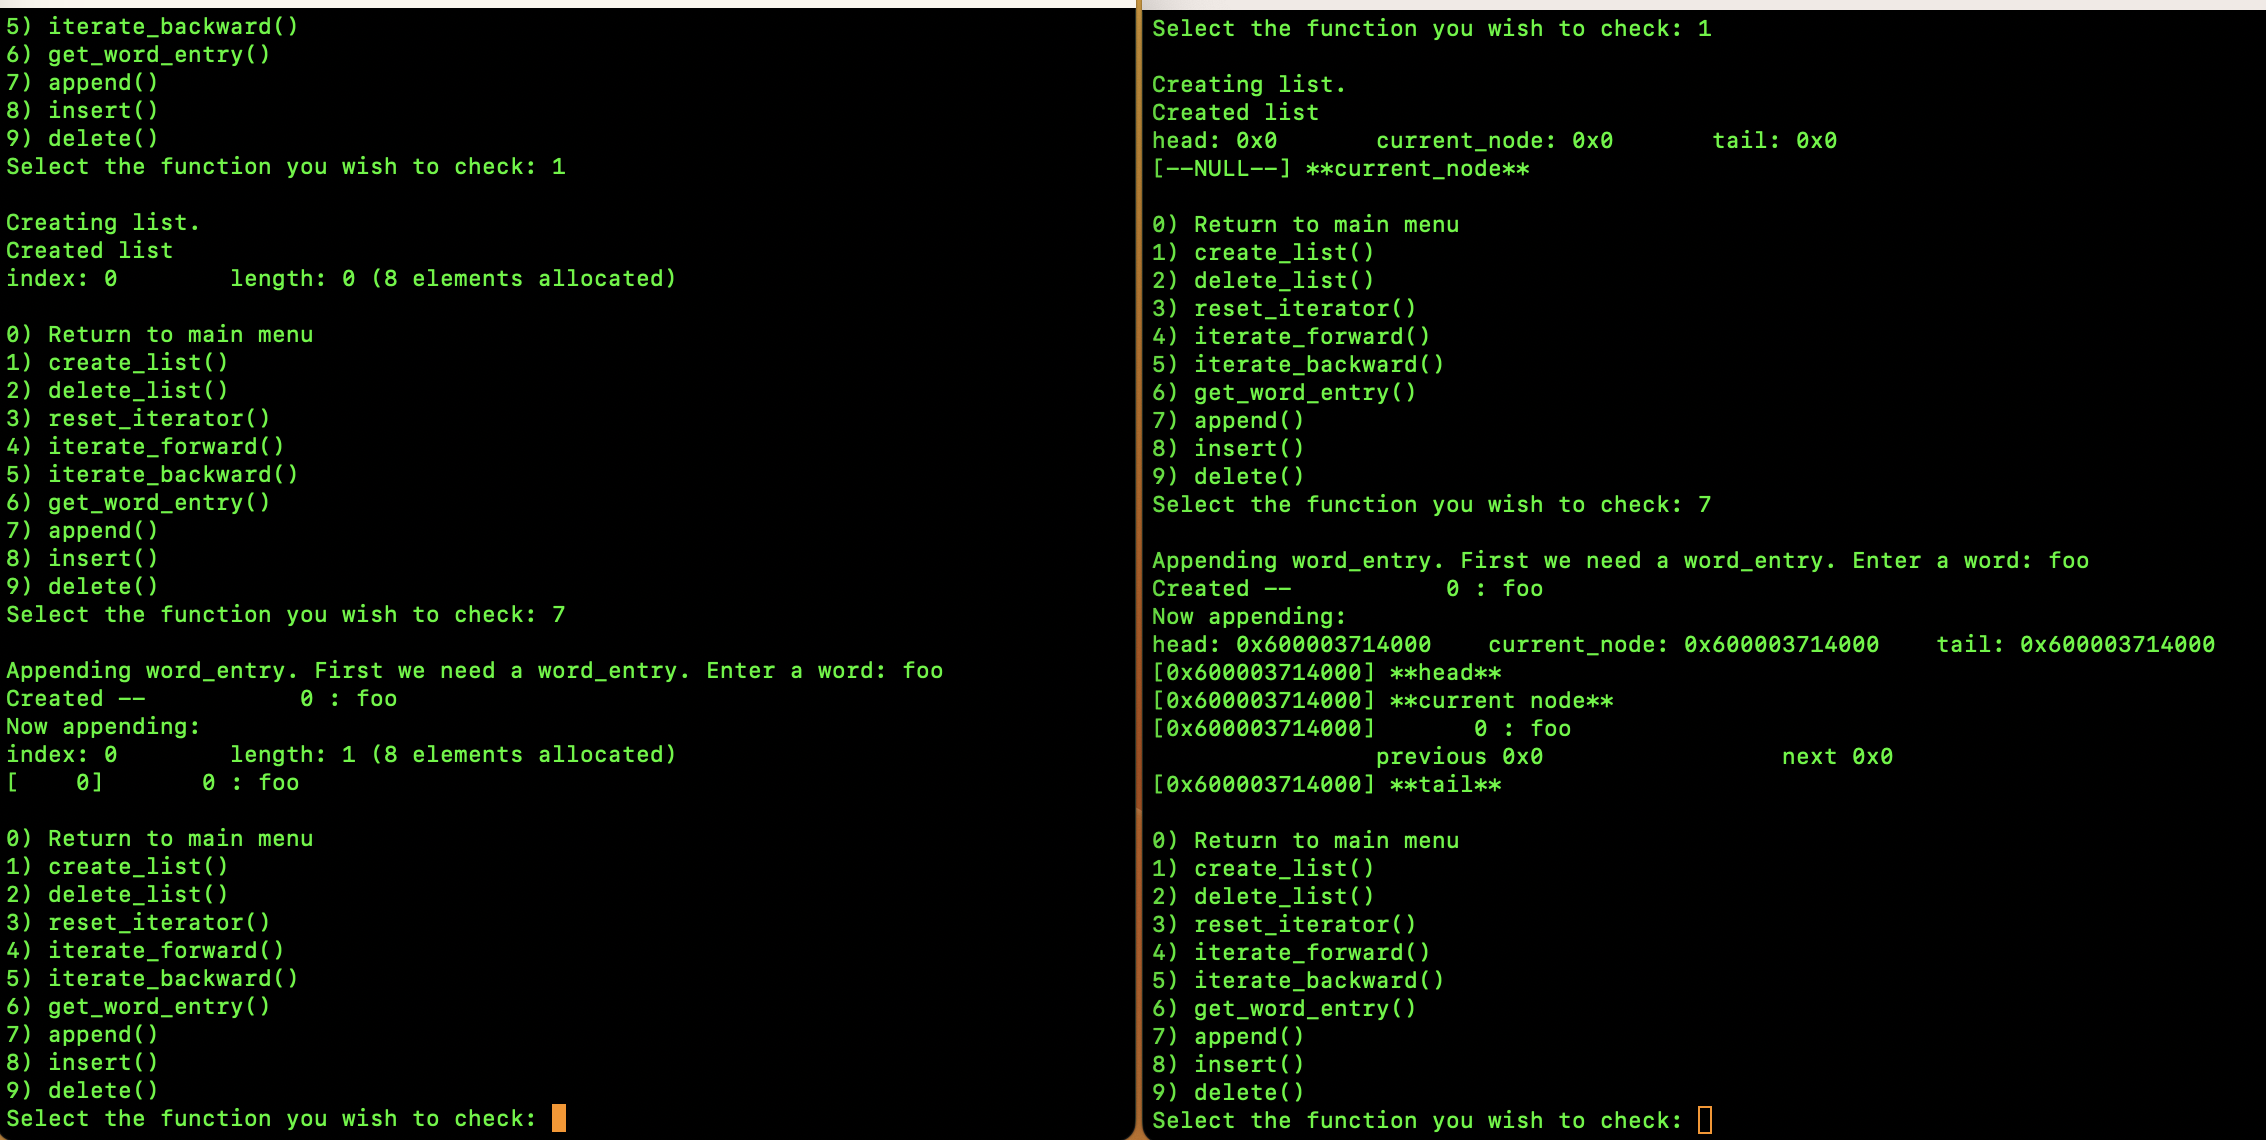
\includegraphics[width=6in]{SideBySideTesting}
    \caption{Testing an array-backed list (left) and a linked list (right) side-by-side.}
    \label{fig:SideBySideTesting}
\end{figure}

To test your linked list implementation, run \textit{linkedlistlab} (and, optionally, \textit{arraylistlab} in another terminal window),
and select option 2, ``Test list''


\subsection{Creating a Node, Creating a List}

In \textit{linked\_list.c}:

\begin{description}
    \checkoffitem{Edit \function{create_node()} to initialize all of a new node's fields.}
    \checkoffitem{Edit \function{create_list()} to initialize all of a new list's fields.}
    \checkoffitem{Test \function{create_node()} and \function{create_list()} by selecting option 2 (``Test list'') and function 1 (``create\_list()'').}
    \checkoffitem{Free the memory by selecting function 2 (``delete\_list()'').
        Exit out of the program by selecting function 0, then option 0.}
\end{description}

It is unlikely that you made any errors that would cause the ``create\_list()'' test to fail,
but it's better to find out now if you did.


\subsection{Appending a Node}

The \function{append()} function takes a word entry, makes it the payload of a new node, and places the new node at the end of the linked list.
The new node, of course, becomes the tail of the list.
If the list is initially empty, then the new node is also the head of the list.

\begin{description}
    \checkoffitem{Edit \function{append()} to place a word entry at the end of the list.}
    \checkoffitem{Create a list by selection option option 2 (``Test list'') and function 1 (``create\_list()'').}
    \checkoffitem{Test \function{append()} for an empty list by selecting function 7 (``append()'').}
    \checkoffitem{Test \function{append()} for a list with one node by selecting function 7 (``append()'').}
    \checkoffitem{Test \function{append()} for a list with multiple nodes by selecting function 7 (``append()'').}
    \checkoffitem{Free the memory by selecting function 2 (``delete\_list()'').
        Exit out of the program by selecting function 0, then option 0.}
\end{description}


\subsection{Iterator Manipulation}

The \function{reset_iterator()} function should make the iterator point to the first element in the sequence.
For a linked list, this means that the current node should be the head.
If successful, then the function returns \lstinline{true},
but if there isn't a first element (that is, if the head is \lstinline{NULL}) then the function returns \lstinline{false}.

The \function{iterate_forward()} and \function{iterate_backward()} functions cause the iterator to move back and forth across the sequence.
For a linked list, this means that you follow the current node's \lstinline{next} or \lstinline{previous} pointers, as appropriate.

\begin{description}
    \checkoffitem{Implement \function{reset_iterator()}.}
    \checkoffitem{Implement \function{iterate_forward()}.}
    \checkoffitem{Implement \function{iterate_backward()}.}
    \checkoffitem{Create a list by selection option option 2 (``Test list'') and function 1 (``create\_list()'').}
    \checkoffitem{Test these functions on an empty list by selecting function 3 (``reset\_iterator()''), function 4 (``iterate\_forward()''), and function 5 (``iterate\_backward()'').
        The test should state that the iterator doesn't change for any of these functions.}
    \checkoffitem{Create a list with one node by selecting function 7 (``append()'').}
    \checkoffitem{Test these functions on a singleton list by selecting function 3 (``reset\_iterator()''), function 4 (``iterate\_forward()''), and function 5 (``iterate\_backward()'').
        Pay attention to whether the test states that the iterator changed or not.
        When the iterator does change, you should also see that the address of the current node has changed.}
    \checkoffitem{Create a list with multiple nodes by selecting function 7 (``append()'').}
    \checkoffitem{Continue to test the iterator manipulation functions until you discover a bug or are satisfied that your implementations are correct.}
    \checkoffitem{Free the memory by selecting function 2 (``delete\_list()'').
        Exit out of the program by selecting function 0, then option 0.}
\end{description}


\subsection{Examining Word Entries}

The \function{get_word_entry()} function retrieves the current node's word entry.
The \function{get_first_word_entry()} and \function{get_last_word_entr()} retrieve the head's and tail's word entries, respectively.
If the current, head, or tail pointers are \lstinline{NULL}, then the corresponding functions return \lstinline{NULL}.

\begin{description}
    \checkoffitem{Implement \function{get_word_entry()}.}
    \checkoffitem{Implement \function{get_first_word_entry()}.}
    \checkoffitem{Implement \function{get_last_word_entry()}.}
    \checkoffitem{Create a list by selection option option 2 (``Test list'') and function 1 (``create\_list()'').}
    \checkoffitem{Test \function{get_word_entry()} on an empty list by selecting function 6 (``get\_word\_entry()'').}
    \checkoffitem{Create a list with one node by selecting function 7 (``append()'').}
    \checkoffitem{Test \function{get_word_entry()} on a singleton list.
        Test it with the iterator pointing at the only node in the list,
        and test it with the iterator pointing at the ```empty'' space after the word entry}
    \checkoffitem{Create a list with multiple nodes by selecting function 7 (``append()'').}
    \checkoffitem{Continue to test \function{get_word_entry()} until you discover a bug or are satisfied that your implementation is correct.}
    \checkoffitem{Free the memory by selecting function 2 (``delete\_list()'').
        Exit out of the program by selecting function 0, then option 0.}
\end{description}


\subsection{Inserting a Node}

The \function{insert()} function takes a word entry, makes it the payload of a new node, and places the new node before the current node and after the current node's predecessor node.
The new node, becomes the current node.
There are a couple of special cases:
\begin{itemize}
    \item If the list is initially empty, then the new node is also the head and the tail of the list.
    \item If the current node is \lstinline{NULL} but there is head and tail, then the iterator points at the ``empty'' space after the last word entry.
        In this case, the new node is also the tail.
\end{itemize}

\begin{description}
    \checkoffitem{Implement \function{insert()}.
        Be sure to handle its special cases.}
    \checkoffitem{Create a list by selection option option 2 (``Test list'') and function 1 (``create\_list()'').}
    \checkoffitem{Test \function{insert()} on an empty list by selecting function 8 (``insert()'').}
    \checkoffitem{Thoroughly test \function{insert()} until you discover a bug or are satisfied that your implementation is correct.
        (Use the iterator manipulation functions to move the iterator to where it needs to be for each test.)}
    \checkoffitem{Free the memory by selecting function 2 (``delete\_list()'').
        Exit out of the program by selecting function 0, then option 0.}
\end{description}


\subsection{Deleting a Node} \label{subsec:DeletingNode}

The \function{delete()} function removes and deletes the current node from the list, updating its neighbors' \lstinline{next} and \lstinline{previous} pointers (and possibly the list's \lstinline{head} or \lstinline{tail} pointer) accordingly.
After the deletion, the deleted node's successor node becomes the current node.
\begin{itemize}
    \item[] \textit{Exception} -- if the deleted node was the list's tail, then that node's ``successor'' is the ``empty'' space after the last word entry.
        In this case, the new tail should become the current node.
    \item[] \textit{Exception to the exception} -- if the deleted node was the only node in the list, then there isn't a new tail, and so the current node is \lstinline{NULL}.
\end{itemize}

\begin{description}
    \checkoffitem{Implement \function{delete()}.
        Be sure to handle its special cases.}
    \checkoffitem{Create a list by selection option option 2 (``Test list'') and function 1 (``create\_list()'').}
    \checkoffitem{Populate the list with several using \function{append()} and/or \function{insert()}.}
    \checkoffitem{Thoroughly test \function{delete()} (function 9) until you discover a bug or are satisfied that your implementation is correct.
        (Use the iterator manipulation functions to move the iterator to where it needs to be for each test.
        Place more word entries in the list if  you need to.)}
    \checkoffitem{Free the memory by selecting function 2 (``delete\_list()'').
    Exit out of the program by selecting function 0, then option 0.}
\end{description}


When you are satisfied that your linked list functions are correct, test their integration into the challenge-response system.
You can use the ``\textit{file}-table.md'' files to confirm the correctness of the results.

\textcolor{red}{If your program requires more than a few seconds to build a list, or does not get a challenge word's response nearly instantaneously, then there is a bug in your code.}

\begin{description}
    \checkoffitem{Test building a list until you discover a bug or are satisfied that your implementations are correct.}
    \checkoffitem{Test challenge/responses until you discover a bug or are satisfied that your implementations are correct.}
    \checkoffitem{When you have finished, select 0 to exit the program.}
\end{description}

As a reminder, the book files are:

\begin{itemize}
    \item ``Animals'' (sorted, 7 words)
    \item ``Plants'' (unsorted, 7 words)
    \item ``Cars'' (sorted, 74 words)
    \item ``Food'' (unsorted, 125 words)
    \item ``Frankenstein'' (sorted, 74,363 words)
    \item ``TheLostWorld'' (unsorted, 77,268 words)
\end{itemize}

Your code might already be able to handle large files in just a few seconds, in which case you are finished.

On the other hand, your code might run briskly when working with smaller files of only a couple of hundred words but then become very sluggish when the number of words is in the thousands.
This tends to be due to one (or both) of two causes.
Look for inefficient algorithms, and look for memory leaks.
If you use the \texttt{top} utility while running your program, and you notice that your program is allocating more than 10MB, then you probably have a memory leak.
If your program is allocating more than 1GB, then your program most certainly has a memory leak.


    \section{Turn-in and Grading}                                   \filesubmission.

\policyforcodethatdoesnotcompile

\latepolicy

\subsection*{Rubric}

This assignment is worth 35 points.
\begin{description}
    \rubricitem{1}{\function{is_nan()} correctly reports whether or not its argument is a number}
    \rubricitem{1}{\function{is_zero()} correctly reports whether or not its argument is zero}
    \rubricitem{1}{\function{is_infinity()} correctly reports whether or not its argument is infinite}
    \rubricitem{1}{\function{is_negative()} correctly reports whether or not its argument is negative}
    \rubricitem{1}{\function{get_754_integer()} correctly extracts the significand's implicit integer}
    \rubricitem{1}{\function{get_754_fraction()} correctly extracts the significand's fraction bits}
    \rubricitem{1}{\function{get_754_exponent()} correctly extracts the exponent}
    \rubricitem{1}{\function{decode()} correctly converts an \lstinline{ieee754_t} value into a \lstinline{unnormal_t} structure}
    \rubricitem{1}{\function{negate()} correctly changes its argument's sign}
    \rubricitem{5}{\function{add()} can add integers \& fractions, positive \& negative values, and ``large'' \& ``small'' numbers}
    \rubricitem{1}{The identity and commutative properties hold for \function{add()}}
    \rubricitem{1}{\function{add()} provides correct answers for its special cases}
    \rubricitem{5}{\function{multiply()} can multiply integers \& fractions, positive \& negative values, and ``large'' \& ``small'' numbers}
    \rubricitem{2}{The identity, zero, and commutative properties hold for \function{multiply()}}
    \rubricitem{1}{\function{multiply()} provides correct answers for its special cases}
    \rubricitem{1}{\function{divide()} provides correct answers for its special cases}
    \rubricitem{1}{\function{divide()} can divide when the divisor is of the form $\pm 2^n, -126 \le n \le 127$}
    \rubricitem{1}{\function{divide()} can divide when the dividend's significand is a multiple of the divisor's significand}
    \rubricitem{1}{\function{add()} demonstrates that \function{encode()} rounds down when the truncated part of the significand is less than halfway between representable values}
    \rubricitem{1}{\function{add()} demonstrates that \function{encode()} rounds up when the truncated part of the significand is more than halfway between representable values}
    \rubricitem{2}{\function{add()} demonstrates that \function{encode()} rounds to the nearest-even when the truncated part of the significand is exactly halfway between representable values}
    \rubricitem{1}{Rounding can carry into the exponent}
    \rubricitem{1}{\function{add()} and/or \function{multiply()} demonstrate that \function{encode()} overflows to infinity}
    \rubricitem{1}{\function{add()}, \function{multiply()}, and/or \function{divide()} demonstrate that \function{encode()} gracefully underflows through subnormal numbers}
    \rubricitem{1}{\function{multiply()} and/or \function{divide()} demonstrate that \function{encode() underflows to zero}}
    \bonusitem{2}{\function{divide()} can divide arbitrary values}
\end{description}

\textbf{Penalties}
\begin{description}
    \softwareengineeringpenalties
    \item[no credit] for functions that use \lstinline{float} or \lstinline{double} variables or constants, use \lstinline{union} variables, use C's floating point operations, and/or a function you did not write
    \item[no credit] for arithmetic functions, if \function{decode()} and/or \function{encode()}  use \lstinline{float} or \lstinline{double} variables or constants, use \lstinline{union} variables, use C's floating point operations, and/or a function you did not write
\end{description}


    \section*{Epilogue}                                             \scenariowrapup

    \textit{To be continued\dots}

    \newpage\appendix

    \section{Appendix: Differences and Similarities between Java and C that are Relevant to this Assignment}
                                                                    In some regards, Java keeps things simple: every variable is a reference, except when it isn't.
In other regards, C keeps things simple: you always know whether the variable you're using is a value or a pointer.

\subsection{Comparing Strings}

You probably learned that when comparing Java Strings, using the equality operator \lstinline{==} is error-prone.
When comparing two String literals (or variables assigned to String literals), the equality operator usually acts as a naive programmer would expect:
\lstinline{"abc" == "abc"} evaluates to \lstinline{true}.
When one or both of the Strings are generated at runtime, such as from user input, then the equality operator rarely evaluates to \lstinline{true}:
\lstinline{userInput == "abc"} will evaluate to \lstinline{false} even when the user entered ``abc''.

The reason for this is that when comparing objects (other than boxed types), Java's comparators compare the objects' references;
that is, Java comparators compare the objects' memory addresses.
Using the \lstinline{==} operator to compare Strings evaluates to \lstinline{true} only when the two Strings occupy the same address;
that is, they are both literally the same String object.
This is why you were taught to use Java's \function{String.equals()} method to compare strings.

Comparing C strings' variables has the same pitfall:
because the string variables are pointers to the first character in their respective strings, using arithmetic comparators will compare the strings' addresses.
If you want to compare two C strings, you would use the \function{strcmp()}\footnote{See footnote~\ref{note:stringFunctions}.} function.
The wrinkle is that \function{strcmp()} returns \lstinline{0} (\textit{i.e.}, \lstinline{false}) when the two strings are equal;
you will often see the idiom \lstinline{if (!strcmp(string1, string2)) {}.

The \function{strcmp(string1, string2)} function actually performs a lexicographic comparison of the strings, returning a negative value if \lstinline{string1} occurs alphabetically earlier than \lstinline{string2}, zero if every character in the two strings match, and a positive value if \lstinline{string1} occurs alphabetically later than \lstinline{string2}.
In this regard, C's \function{strcmp()} function is more like Java's \function{String.compareTo()} method than \function{String.equals()}.

\subsection{Copying Strings}

Because Java Strings are immutable objects, you can safely copy a string by simply copying its reference (this is called \textit{aliasing}).
You can safely write the statement \lstinline{string1 = string2;} without worrying about changes to \lstinline{string2} causing changes in \lstinline{string1}
(if you were to make changes to \lstinline{string2}, it would result in a new String object being assigned to the \lstinline{string2} variable).

For mutable objects, creating an alias (that is, copying the reference) results in the situation that changes made through one variable are visible through the other variable.
For example, if you have the statements \lstinline{list1 = list2; list2.add(foo);} then \\ \lstinline{list1.size() == list2.size() && list1.contains(foo)} will evaluate to \lstinline{true}.
If the object's class implements the \lstinline{Cloneable} interface then you can make a copy of an object without aliasing it.
If you have the statements \lstinline{list1 = list2.clone(); list2.add(foo);} then \lstinline{list1.size() == list2.size()} will evaluate to \lstinline{false}.

In general, C strings are mutable.\footnote{
    The exceptions are string literals, which are immutable, and strings declared as a pointer to a constant, which if treated as mutable will result in undefined behavior.
}
This means that you generally don't want to create an alias.\footnote{
    Sometimes you can't create an alias.
    If the left-hand-side of an assignment is a constant pointer or is effectively a constant pointer -- such as an array inside a struct -- then it cannot be re-assigned.
}
Instead, use the \function{strcpy(destination, source)} or \function{strncpy(destination, source, n)}\footnote{See footnote~\ref{note:stringFunctions}.} function to copy the \lstinline{source} string into the memory pointed to by \lstinline{destination}.
The \function{strcpy()} function will continue copying until encountering the terminating \lstinline{NUL} in the \lstinline{source} string -- this is very slightly faster (not enough that you'd notice) but is safe only if you can prove that \lstinline{destination} has enough memory allocated for the string.
The \function{strncpy()} function will copy until encountering the terminating \lstinline{NUL} or until it has copied $n-1$ characters (after which it will append a terminating \lstinline{NUL}) -- this is safer because you can ensure that the string copied to \lstinline{destination} will fit within the space allocated for it.

\subsection{Allocating and Deallocating Memory}

Java's \lstinline{new} keyword allocates space for the new object, inferring the amount of space needed based on the class's definition.
In C, you use the \function{malloc()} function to allocate space\footnote{
    There are a small handful of alternate functions, each with their own use cases, but \function{malloc()} is most-suitable for this lab.
}, and you must be explicit about how much space you need.
An idiom is to combine \function{malloc()} with the \function{sizeof()} function, as you saw in PokerLab, and as you'll see near the start of Section~\ref{subsubsec:cImplementation}.

Java uses a \textit{garbage collector} to reclaim memory allocated for objects that are no longer in use.
The unpredictability of when garbage collection happens makes an automatic garbage collector unsuitable for many of C's uses.
For this reason (among others), the programmer is responsible for deallocating memory that is no longer needed.
This is done with the \function{free()} function.

While a variable will go out of scope at the end of the code block in which it was declared, memory allocated in that code block persists unless explicitly \function{free}d.
Once the last pointer pointing to that memory goes out of scope, you no longer have a way to \function{free} that memory, resulting in a \textit{memory leak}.
On the other hand, \function{free}ing memory while it is still being used by another pointer can result in undefined behavior.
This requires careful thought to make sure that you \function{free} all memory that you allocated, but only after it is safe to do so.

For many short-running programs, such as those you often write in school, you often can ignore the need to \function{free} allocated memory since all the program's memory will be reclaimed by the operating system when the program terminates.
A member of the C Standard Committee recently described this as having a maid that will clean up your mess.\footnote{
    Sarcasm alert: \url{https://twitter.com/__phantomderp/status/1619322783162568705}, \\ \url{https://twitter.com/__phantomderp/status/1619323139665846273}
}

I advise you not to rely on that ``maid'' even for a ``short-running program,'' such as this one.
In an earlier version of this lab, there were a dozen or so students whose code, when tested against a 75,000-word file, would quickly consume all the server's physical memory.
As the first of these programs thrashed the virtual memory system, it prevented other services from working effectively, including the one that I had precautionarily introduced to kill a test after a couple of minutes.
It consumed enough resources that the system administrator couldn't log in to determine why the server had slowed to a crawl.
As I was already logged in, I was able to kill the process as the system administrator was preparing to disconnect the server from the power line.
The system administrator later commented about the resources it consumed, ``You ought never to see a `T' in the memory column'' (Figure~\ref{fig:tooMuchMemoryUsed}).

\begin{figure}
    \center
    % TODO -- get this file
%    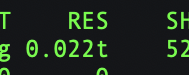
\includegraphics{too-much-memory-used}
    \caption{Screenshot showing a student's program consuming 0.022 terabytes of physical memory;
    the allocated virtual memory is not visible in the image.\label{fig:tooMuchMemoryUsed}}
\end{figure}

%\subsubsection{Idioms for Defining and Initializing \texttt{Struct} Types}
%
%In PokerLab, you worked with a struct that was defined by \lstinline{typedef} as a new type.
%In this lab, you will work with a struct defined simply as a \lstinline{struct}, without a \lstinline{typedef}.
%There are compelling arguments for and against both approaches in different use cases.
%You should learn to be comfortable with both approaches.
%
%In this lab, the function that initializes a node is also responsible for allocating space for that node.
%In PokerLab, you saw the other idiom, in which the calling function is responsible for allocating space and passing the pointer to the initializer (this pointer is analogous to Java's implicit \lstinline{this} parameter).
%The approach of having the caller allocate space seems to be more common, but both approaches are common enough to be aware of both.
%(The third idiom is not to have a separate initializing function;
%I discourage this approach.)

\subsection{Declaration vs Definition}

In C, types, variables, and functions must be \textit{declared} earlier in the file (or in an \lstinline{#include}d file) than their first use;
however, they typically do not need to be \textit{defined} until later.
A declaration provides establishes the existence and scope, and it provides enough information for the compiler to check for mismatches.
For example, a function ``prototype'' commonly found in header files simply provides the name of a function and its signature.
You can have arbitrarily many declarations for the same entity as long as they don't conflict with each other.

A definition, on the other hand, provides all the details.
(A definition is also implicitly a declaration.)
For example, a function's definition has all of its code.
An entity can only have one definition within its scope.
Functions, for example, typically have global scope, and so you cannot have multiple functions with the same name, even if they're in different files.

You are more likely, by far, to see function declarations that are not definitions than you are to see anything else declared without a definition.
In a future lab, you'll see an example of a variable declaration that has its definition in a separate file.

In this lab, we have an example of a type declaration that occurs separately from its definition.
In \textit{list.h.}, we declare a \lstinline{struct list_definition} type (and \lstinline{typedef} it to \lstinline{list_t}) without a definition.
Because none of the function prototypes in \textit{list.h} need to know anything about \lstinline{list_t} other than its existence, and because none of the code in \textit{challenge-response.c} depends on the definition, you are able to write code for the challenge-response system without regard to the underlying representation.
We provide a definition of \lstinline{struct list_definition} in \textit{array\_list.h} and another definition in \textit{linked\_list.h}.
We crafted the Makefile so that when you build \textit{arraylistlab}, only the definition in \textit{array\_list.h} is included;
similarly, when you build \textit{linkedlistlab}, only the definition in \textit{linked\_list.h} is included.
In doing so, we ensure that each executable has only one definition of \lstinline{struct list_definition}.

Note that the code in \textit{linked\_list.c} does depend on \lstinline{struct list_definition}'s definition, but that's okay because \textit{linked\_list.c} \lstinline{#include}s \textit{linked\_list.h}.


\subsection{The \lstinline{static} Keyword \\ \footnotesize{does not mean what you think it means}}

In Java, the \lstinline{static} keyword is used to make a field or method be shared among all instances of a class, and even be available without having an instance of the class.
The C programming language doesn't have classes, so clearly \lstinline{static} cannot mean the same thing.

In C, \lstinline{static} can be used in two different ways.
In a future lab, we'll see the use of \lstinline{static} for function-scoped variables.
In this lab, we have two functions in \textit{linked\_list.c} that are modified with the \lstinline{static} keyword.

When function or variable that is declared outside of any function is modified with the \lstinline{static} keyword, it no longer has global scope;
instead, its scope is limited to the file.
You can think of it as roughly corresponding to Java's \lstinline{private} visibility modifier.
This has two implications:
\begin{itemize}
    \item A file-scoped function or variable cannot be accessed from code in another file
    \item Another file-scoped function or variable of the same name can be defined in another file without violating the rule against multiple definitions
\end{itemize}


    \section{Appendix: Linked Lists}                                You probably learned about linked lists in \cstwo; however, we will provide a refresher.

A \textit{linked list} is a linear collection of data.
Like an array, each element (or \textit{node}) has a particular position in the list, and when you iterate over the list, you always access the elements in the same order every time (unless you change or re-order the elements).

In an array, the elements are contiguous in memory, and you can access a specific element by indexing the array (or, equivalently, performing pointer arithmetic).
In a linked list, however, the nodes can be in arbitrary locations in memory, and the nodes are connected by references (in C, pointers).
You can access a specific element only by following pointers from one node to the next until you reach the desired node.


\subsection{Singly-Linked List} \label{subsec:singlylinkedlist}

The simplest linked list is a \textit{singly-linked list}.
A node consists of a \textit{payload} (the data that we care about) and a reference to the \textit{next} node;
see Figure~\ref{fig:singly-linked-list}.

\begin{figure}[h]
    \centering
    \begin{tikzpicture}[x=1.5mm, y=1.5mm]
        \draw[-stealth,very thick,magenta](-19,-3) -- (-10,0);
        \sllnode{0}{0}{0}
        \draw[-stealth,very thick,magenta](5,-5) -- (20,0);
        \sllnode{30}{0}{0}
        \draw[-stealth,very thick,magenta](35,-5) -- (50,0);
    \end{tikzpicture}
    \caption{Nodes in a singly-linked list consist of the payload data and a reference that points to the next node.}\label{fig:singly-linked-list}
\end{figure}

A linked list's greatest advantage over an array is that inserting and removing a node at an arbitrary location takes constant time, whereas inserting an element into an array (assuming there is sufficient memory allocated for the array) or removing an element from an array requires moving all the elements that follow the element's index.
Inserting a new node, $C$, between adjacent nodes $A$ and $B$ (where $B = A.next$) requires connecting $C.next$ to $B$ and re-assigning $A.next$ to $C$;
see Figure~\ref{fig:sll-insertion}.

\begin{figure}[h]
    \centering
    \begin{tikzpicture}[x=1.5mm, y=1.5mm]
        \draw[-stealth,very thick,magenta](-19,-3) -- (-10,0);
        \sllnode{0}{0}{0}
        \draw[-stealth,very thick,magenta](5,-5) -- (13,-5) -- (13,-12.5) -- (0,-12.5) -- (0,-25) -- (5,-25);
        \sllnode{15}{-25}{0}
        \draw[-stealth,very thick,magenta](20,-30) -- (30,-30) -- (30,-12.5) -- (17,-12.5) -- (17,0) -- (20,0);
        \sllnode{30}{0}{0}
        \draw[-stealth,very thick,magenta](35,-5) -- (50,0);
    \end{tikzpicture}
    \caption{Inserting a new node into a singly-linked list only requires assignments to the affected \textit{next} pointers.}\label{fig:sll-insertion}
\end{figure}

As with an array, you do need to maintain a variable that points to the list.
Conventionally, this is a reference to the \textit{head} of the list.
(Note that if a new node is inserted before the current head node, then the new node becomes the head of the list, and your \lstinline{head} variable would need to be updated.)
It is not uncommon to also maintain a reference to the \textit{tail} of the list.

%\subsection{Circular Linked List} \label{subsec:circularlinkedlist}
%
%A \textit{circular linked list} is a linked list in which the tail's \textit{next} field points to the head of the list.
%In essence, a circular linked list has no head (because every node is some node's \textit{next}), and has no tail (because every node's \textit{next} is non-NULL);
%see Figure~\ref{fig:circular-linked-list}.
%
%\begin{figure}[h]
%    \centering
%    \begin{tikzpicture}[x=1.5mm, y=1.5mm]
%        \sllnode{0}{30}{0}
%        \draw[-stealth,very thick,magenta,rotate=0](5,25) -- (25.5,18.8);
%        \sllnode{0}{30}{-72}
%        \draw[-stealth,very thick,magenta,rotate=-72](5,25) -- (25.5,18.8);
%        \sllnode{0}{30}{-144}
%        \draw[-stealth,very thick,magenta,rotate=-144](5,25) -- (25.5,18.8);
%        \sllnode{0}{30}{144}
%        \draw[-stealth,very thick,magenta,rotate=144](5,25) -- (25.5,18.8);
%        \sllnode{0}{30}{72}
%        \draw[-stealth,very thick,magenta,rotate=72](5,25) -- (25.5,18.8);
%    \end{tikzpicture}
%    \caption{A circular linked list does not have a well-defined head and tail.}\label{fig:circular-linked-list}
%\end{figure}
%
%You still need to maintain a variable that points to \textit{some} node in the list.


\subsection{Doubly-Linked List} \label{subsec:doublylinkedlist}

A \textit{doubly-linked list} is a linked list with the property that each node maintains a link not only to the \lstinline{next} node but also a link to the \lstinline{previous} node.
In C, these links are pointers.

\begin{figure}[h]
    \centering
    
\begin{tikzpicture}[x=1.5mm, y=1.5mm]
        \draw[-stealth,very thick,magenta](-20,-4.25) -- (-10,0);
        \draw[stealth-,very thick,yellow](-20,0) -- (-8,-5);
        \dllnode{0}{0}{0}
        \draw[-stealth,very thick,magenta](8,-5) -- (20,0);
        \draw[stealth-,very thick,yellow](10,0) -- (22,-5);
        \dllnode{30}{0}{0}
        \draw[-stealth,very thick,magenta](38,-5) -- (50,0);
        \draw[stealth-,very thick,yellow](40,0) -- (50,-4.25);
    \end{tikzpicture}
    \caption{Nodes in a doubly-linked list consist of the payload data and references that point to the previous and next nodes.}\label{fig:doubly-linked-list}
\end{figure}

Inserting new node, $C$, between adjacent nodes $A$ and $B$ (where $B = A.next$ and $A = B.previous$) requires connecting $C.previous$ to $A$ and $C.next$ to $B$, and re-assigning $A.next$ to $C$ and $B.previous$ to $C$.



\subsection{Equivalent Java Code} \label{subsec:equivalentjava}

In Java, you probably wouldn't implement your own linked list;
instead, you would use \lstinline{java.util.LinkedList}, which has been available since J2SE~1.2.
%(ignoring for the moment that Java's standard library doesn't have a circular linked list).
A list of \lstinline{WordEntry} objects would be created with:
\begin{lstlisting}[numbers=none]
    List<WordEntry> wordEntries = new LinkedList<>;
\end{lstlisting}

C doesn't have a built-in linked list data type, so you will need to design one.
Let us consider what a custom linked list would look like in Java.

\begin{lstlisting}[mathescape=true]
public class WordEntry {
    private final String word;          $\label{code:javaWord}$
    private int occurrences;            $\label{code:javaOccurrences}$ $\lstsetnumber{\ldots}$
    ...$\lstresetnumber\setcounter{lstnumber}{53}$
}
\end{lstlisting}

\begin{lstlisting}[firstnumber=100, mathescape=true]
public class Node {
    private final WordEntry wordEntry;  $\label{code:javaPayload}$
    private Node next;                  $\label{code:javaNext}$
    private Node previous;              $\label{code:javaPrevious}$

    public Node(WordEntry wordEntry) {$\lstsetnumber{\ldots}$
        ...$\lstresetnumber\setcounter{lstnumber}{111}$
    }
    $\lstsetnumber{\ldots}$
    ...$\lstresetnumber\setcounter{lstnumber}{203}$
}
\end{lstlisting}

\begin{lstlisting}[firstnumber=309, mathescape=true]
public class MyIterator {
    private MyLinkedList list;
    private Node currentNode;
    $\lstsetnumber{\ldots}$

    public MyLinkedList insert(WordEntry wordEntry) {
        Node node = new Node(wordEntry){$\lstsetnumber{\ldots}$
        ...$\lstresetnumber\setcounter{lstnumber}{329}$
    }
    $\lstsetnumber{\ldots}$
    ...$\lstresetnumber\setcounter{lstnumber}{417}$
\end{lstlisting}

\begin{lstlisting}[firstnumber=452, mathescape=true]
public class MyLinkedList {
    private Node head;
    private Note tail;
    private Node current;

    public MyIterator append(WordEntry wordEntry) {
        Node node = new Node(wordEntry){$\lstsetnumber{\ldots}$
        ...$\lstresetnumber\setcounter{lstnumber}{473}$
    }
    $\lstsetnumber{\ldots}$
    ...$\lstresetnumber\setcounter{lstnumber}{528}$
}
\end{lstlisting}

Creating and inserting a new word entry would look something like this:

\begin{lstlisting}[firstnumber=642, mathescape=true]
    iterator = list.append(new WordEntry("eggplant"));
    while (...) iterator.swapPrevious(); // determine where new node goes
    if (...) iterator.merge();           // no duplicate word entries allowed
\end{lstlisting}
%WordEntry wordEntry = new WordEntry("eggplant");    $\label{code:newWordEntry}$
%list.insert(wordEntry);                             $\label{code:javaInsert}$

Recall that in Java, all variables except primitive types (such as \lstinline{occurrences} on line~\ref{code:javaOccurrences}) are references.
This means that the \lstinline{next} field on line~\ref{code:javaNext} is a reference to another Node, just as we described in Section~\ref{subsec:singlylinkedlist}.
The payload is the \lstinline{wordEntry}.

\subsubsection{C Implementation} \label{subsubsec:cImplementation}

In \textit{linked-list.h}, you'll see \lstinline{struct}s fields similar to our Java example
(we've placed the pointer to the current node in an iterator to make the mental model for some of the operations more explicit):

\lstinputlisting[linerange=41-45, firstnumber=41]{../starter-code/linked_list.h}

\lstinputlisting[linerange=58-60, firstnumber=58]{../starter-code/linked_list.h}

\lstinputlisting[linerange=71-74, firstnumber=71]{../starter-code/linked_list.h}

In \textit{linked\_list.c}, you'll also see the \function{create_node()} and \function{create_list()} functions:

\lstinputlisting[linerange=36-41, firstnumber=36]{../starter-code/linked_list.c}

\lstinputlisting[linerange=74-79, firstnumber=74]{../starter-code/linked_list.c}

As you can see, they allocate space for a new node or a new list handle using \function{malloc()}.
The code that you will need to add to \function{create_node()} will copy the \lstinline{word_entry} argument into the \lstinline{word_entry} field.
Since we don't yet know where this node will go, set the node's \lstinline{next} and \lstinline{previous} pointers to point to NULL\@.
The code that you will need to add to \function{create_list()} is even simpler: a newly-created list is empty, and so it has no head, no tail, and no current node.


\subsection{A Visualization of the Data Types}

\subsubsection{word\_entry\_t}

\begin{tikzpicture}[x=1.5mm, y=1.5mm]
    \draw[thick] (0,0) rectangle (49,18);
    \draw (17,16) rectangle ++(6,-6) +(-6,3) node[anchor=east] {word};
    \draw (23,16) rectangle ++(6,-6) rectangle ++(6,6) +(3,-3) node {...};
    \draw (41,16) rectangle ++(6,-6);
    \draw (17,8) rectangle ++(6,-6) +(-6,3) node[anchor=east] {occurrences};
\end{tikzpicture}

\subsubsection{node\_t}

\begin{tikzpicture}[x=1.5mm, y=1.5mm]
    \draw[thick] (0,0) rectangle (25,26);
    \draw (17,24) rectangle ++(6,-6) +(-6,3) node[anchor=east] {word\_entry};
    \draw (17,16) rectangle ++(6,-6) +(-6,3) node[anchor=east] {next};
    \draw (17,8) rectangle ++(6,-6) +(-6,3) node[anchor=east] {previous};

    \draw (40,24) rectangle ++(+10,-6) +(-5,3) node (word) {\tiny{word\_entry\_t}};
    \draw[Circle-Stealth,very thick] (20,21) -- (word.west);
    \draw (40,16) rectangle ++(6,-6) +(-3,3) node (next) {\tiny{node\_t}};
    \draw[Circle-Stealth,very thick] (20,13) -- (next.west);
    \draw (40,8) rectangle ++(6,-6) +(-3,3) node (previous) {\tiny{node\_t}};
    \draw[Circle-Stealth,very thick] (20,5) -- (previous.west);
\end{tikzpicture}

\subsubsection{list\_t as an array-backed list}

\begin{tikzpicture}[x=1.5mm, y=1.5mm]
    \draw[thick] (0,0) rectangle ++(25,34);
    \draw (17,32) rectangle ++(6,-6) +(-6,3) node[anchor=east] {array};
    \draw (17,24) rectangle ++(6,-6) +(-6,3) node[anchor=east] {length};
    \draw (17,16) rectangle ++(6,-6) +(-6,3) node[anchor=east] {allocation};
    \draw (17,8)  rectangle ++(6,-6) +(-6,3) node[anchor=east] {iterator};
    \draw[Circle-Stealth,very thick] (20,5) -- (20,-8);

    \draw[thick] (0,-8) rectangle ++(25,-13);
    \draw (17,-10) rectangle ++(6,-6) +(-3,0) node[anchor=north] {index};
    \draw (2,-10) rectangle ++(6,-6) +(-3,0) node[anchor=north] {list};
    \draw[Circle-Stealth,very thick] (5,-13) -- (5,0);

    \draw[Circle-Stealth,very thick] (20,29) -- (40,21);
    \draw (40,24) rectangle ++(6,-6) rectangle ++(6,6) rectangle ++(6,-6) ++(6,0) rectangle ++(6,6) +(-9,-3) node {...};
    \draw (70,24) rectangle ++(6,-6) ++(-3,3) node {X} ++(3,-3) rectangle ++(6,6) ++(-3,-3) node {X} ++(9,-3) rectangle ++(6,6) ++(-3,-3) node {X} +(-6,0) node {...};
    \draw[thin] (40,26) -- ++(0,8) ++(30,-8) -- ++(0,3.5) ++(24,-3.5) -- ++(0,8);
    \draw[<-, thin] (40,28) -- ++(11,0) node[anchor=west] {\footnotesize{length}};
    \draw[->, thin] (40,28) ++(19,0) -- ++(11,0);
    \draw[<-, thin] (40,32) -- ++(21,0) node[anchor=west] {\footnotesize{allocation}};
    \draw[->, thin] (40,32) ++(33,0) -- ++(21,0);

    \draw[Circle-Stealth,very thick] (43,21) -- (38,12);
    \draw (38,12) ++(-5,0) rectangle ++(+10,-6) +(-5,3) node {\tiny{word\_entry\_t}};
    \draw[Circle-Stealth,very thick] (49,21) -- (46,2);
    \draw (46,2) ++(-5,0) rectangle ++(+10,-6) +(-5,3) node {\tiny{word\_entry\_t}};
    \draw[Circle-Stealth,very thick] (55,21) -- (59,15);
    \draw (59,15) ++(-5,0) rectangle ++(+10,-6) +(-5,3) node {\tiny{word\_entry\_t}};
    \draw[Circle-Stealth,very thick] (67,21) -- (80,7);
    \draw (80,7) ++(-5,0) rectangle ++(+10,-6) +(-5,3) node {\tiny{word\_entry\_t}};
\end{tikzpicture}

\subsubsection{list\_t as a linked list} \label{subsubsec:listt-as-lined-list}

\begin{tikzpicture}[x=1.5mm, y=1.5mm]
    \draw[thick] (0,0) rectangle (25,26);
    \draw (17,24) rectangle ++(6,-6) +(-6,3) node[anchor=east] {head};
    \draw (17,16) rectangle ++(6,-6) +(-6,3) node[anchor=east] {tail};
    \draw (17,8)  rectangle ++(6,-6) +(-6,3) node[anchor=east] {iterator};
    \draw[Circle-Stealth,very thick] (20,5) -- (20,-8);

    \draw[thick] (0,-8) rectangle ++(25,-13);
    \draw (17,-10) rectangle ++(6,-6) +(-6,0) node[anchor=north] {current\_node};
    \draw (2,-10) rectangle ++(6,-6) +(-3,0) node[anchor=north] {list};
    \draw[Circle-Stealth,very thick] (5,-13) -- (5,0);

    \draw (38,28) rectangle ++(6,-6) +(-3,3) node (head) {\tiny{node\_t}};
    \draw[Circle-Stealth,very thick] (20,21) -- (head.west);
    \draw (38,16) rectangle ++(6,-6) +(-3,3) node (tail) {\tiny{node\_t}};
    \draw[Circle-Stealth,very thick] (20,13) -- (tail.west);
    \draw (86,4) rectangle ++(6,-6) +(-3,3) node (current) {\tiny{node\_t}};
    \draw[Circle-Stealth,very thick] (20,-13) -- (current.west);

    \draw (38,28)
        ++(12,0) rectangle ++(6,-6) ++(-3,3) node (node1) {\tiny{node\_t}}
        ++(9,3) rectangle ++(6,-6) ++(-3,3) node (node2) {\tiny{node\_t}}
        ++(9,3) rectangle ++(6,-6) ++(-3,3) node (node3) {\tiny{node\_t}}
        ++(9,3) rectangle ++(6,-6) ++(-3,3) node (node4) {\tiny{node\_t}}
        ++(9,3) rectangle ++(6,-6) ++(-3,3) node (node5) {\tiny{node\_t}}
        ++(-3,-9) rectangle ++(6,-6) ++(-3,3) node (node6) {\tiny{node\_t}}
        ++(-3,-9) rectangle ++(6,-6) ++(-3,3) node (node7) {\tiny{node\_t}}
        ++(-15,15) rectangle ++(6,-6) ++(-3,3) node (node8) {\tiny{node\_t}}
        ++(-15,3) rectangle ++(6,-6) ++(-3,3) node (node9) {\tiny{node\_t}}
        ++(-15,3) rectangle ++(6,-6) ++(-3,3) node (node10) {\tiny{node\_t}}
        ++(-15,3) rectangle ++(6,-6) ++(-3,3) node (node11) {\tiny{node\_t}};

    \draw[Stealth-Stealth] (head.east) -- (node1.west);
    \draw[Stealth-Stealth] (node1.east) -- (node2.west);
    \draw[Stealth-Stealth] (node2.east) -- (node3.west);
    \draw[Stealth-Stealth] (node3.east) -- (node4.west);
    \draw[Stealth-Stealth] (node4.east) -- (node5.west);
    \draw[Stealth-Stealth] (node5.south) -- (node6.north);
    \draw[Stealth-Stealth] (node6.south) -- (node7.north);
    \draw[Stealth-Stealth] (node7.west) -- (current.east);
    \draw[Stealth-Stealth] (current.north) -- (node8.south);
    \draw[Stealth-Stealth] (node8.west) -- (node9.east);
    \draw[Stealth-Stealth] (node9.west) -- (node10.east);
    \draw[Stealth-Stealth] (node10.west) -- (node11.east);
    \draw[Stealth-Stealth] (node11.west) -- (tail.east);

    \draw[-Rays] (head.south) -- ++(-5,-3);
    \draw[-Rays] (tail.south) -- ++(5,-3);
\end{tikzpicture}



\end{document}
